
\documentclass[oneside,12pt]{book}

\usepackage[utf8]{inputenc}
\usepackage[greek, english]{babel}

% Packages
\usepackage{alphabeta}
\usepackage{amsmath}
\usepackage{amsthm}
\usepackage{caption}
\usepackage{color}
\usepackage{fullpage}
\usepackage{graphicx}
\usepackage{latexsym}
\usepackage{listings}
\usepackage{pxfonts}
\usepackage{stackrel}
\usepackage{titlesec}
\usepackage{subfig}
\usepackage{tikz}
\usepackage{float}
\usepackage{hyperref}
\usepackage{setspace}
\usepackage{tcolorbox}
\usepackage[ruled,vlined]{algorithm2e}
\tcbuselibrary{theorems}

\addto{\captionsenglish}{\renewcommand{\bibname}{}}
\patchcmd{\thebibliography}{\chapter*}{\section*}{}{}

\newtcbtheorem[number within=section]{mydefinition}{Ορισμός}%
{colback=black!5,colframe=black!15!black,fonttitle=\bfseries}{th}

\newtcbtheorem[number within=section]{mytheorem}{Θεώρημα}%
{colback=black!5,colframe=black!15!black,fonttitle=\bfseries}{th}

\newtcbtheorem[number within=section]{mylemma}{Λήμμα}%
{colback=black!5,colframe=black!15!black,fonttitle=\bfseries}{th}

% Commands
\newcommand{\N}{\mathbb{N}}
\newcommand{\R}{\mathbb{R}}
\newcommand{\code}[2]{\lstinputlisting[caption={#2}]{#1}}
\newcommand{\margin}{\hspace{4pt}}
\newcommand{\norm}[1]{\left\lVert#1\right\rVert}
\newcommand{\abs}[1]{\left\lvert#1\right\rvert}

% Environments
\newenvironment{matlab}
	{\begin{figure}[hp]\centering\captionsetup{justification=centering}}
	{\end{figure}}

\newenvironment{rcases}
	{\left.\begin{aligned}}
	{\end{aligned}\right\rbrace}
% Python Syntax Highlighting
\definecolor{string_color}{RGB}{0, 161, 13}
\definecolor{comment_color}{RGB}{46, 46, 46}
\definecolor{keyword_color}{RGB}{0, 112, 191}
\definecolor{background_color}{RGB}{250, 250, 250}
\lstset{
    framesep=15pt,
    xleftmargin=15pt,
    xrightmargin=15pt,
    language=Python,
    captionpos=b,
    numbers=right,
    numberstyle=\small\ttfamily,
    frame=lines,
    showspaces=false,
    showtabs=false,
    breaklines=true,
    showstringspaces=false,
    breakatwhitespace=true,
    commentstyle=\color{comment_color}\textit,
    keywordstyle=\bfseries\color{keyword_color}\textbf,
    stringstyle=\color{string_color}\textit,
    morekeywords={self, lambda, __init__, __del__, __name__, for, in, not, and, or, :},
    basicstyle=\small\ttfamily,
    tabsize=4,
    keepspaces=true,
    columns=flexible,
    backgroundcolor=\color{background_color}
}
% Links
\hypersetup{
    colorlinks=true,
    linkcolor=blue,
    filecolor=magenta,
    urlcolor=cyan,
}
% Lengths
\setlength{\parindent}{0in}
\setlength{\oddsidemargin}{0in}
\setlength{\textwidth}{6.5in}
\setlength{\textheight}{10in}
\setlength{\topmargin}{-1.0in}
\setlength{\headheight}{18pt}
\setlength{\parskip}{0.3cm}
\setlength{\parindent}{5ex}
\doublespacing
\theoremstyle{definition}
\newtheorem{definition}{Definition}[section]
\titlespacing*{\subsection}
{0pt}{5.5ex plus 1ex minus .2ex}{4.3ex plus .2ex}
\title{\huge Travelling Salesman Problem}
\author{Σιώρος Βασίλειος\\Ανδρινοπούλου Χριστίνα}
\date{Μάϊος 2020}
\begin{document}
\maketitle
\pagenumbering{gobble}
\pagebreak
\tableofcontents

\chapter{Abstract}

\chapter{Introduction}

Το "Travelling Salesman Problem" (TSP) ή με την ελληνική του απόδοση "Πρόβλημα του πλανόδιου πωλητή" (ή εναλλακτικά πρόβλημα του περιοδεύοντος πωλητή) είναι ένα κλασσικό πρόβλημα θεωρητικής επιστήμης των  υπολογιστών. Πρόκειται για ένα πρόβλημα περιήγησης. Ο πωλητής οφείλει να επισκευτεί n το πλήθος πόλεις για να πουλήσει το εμπόρευμά του. Σκοπός του προβλήματος είναι η εύρεση μίας βέλτιστης διαδρομής για τον πωλητή, με την οποία θα μπορέσει να επισκεφτεί όλες τις πόλεις που τον ενδιαφέρουν, μόνο μία φορά την κάθε μία και μάλιστα με τέτοιον τρόπο ώστε να διανύσει τη μικρότερη δυνατή απόσταση. Με άλλα λόγια, ο πωλητής πρέπει να επισκεφτεί την κάθε πόλη ακριβώς μία φορά ακολουθώντας το συντομότερο δρομολόγιο. \\

Το πρόβλημα του περιοδεύοντος πωλητή έχει αποδειχθεί ότι είναι NP-hard (NP-δύσκολο), έννοια την οποία θα αναλύσουμε παρακάτω. Ωστόσο, έχουν γίνει σημαντικές προσπάθειες από την επιστημονική κοινότητα, ώστε οι αλγόριθμοι TSP να βελτιωθούν αισθητά ως προς τις αποδόσεις τους. \\

Φυσικά, το TSP είναι ένα πολύ σημαντικό πρόβλημα στην επιστήμη της πληροφορικής, καθώς έχει μία γκάμα εφαρμογών. Τέτοιες είναι: ο σχεδιασμός των μετακινήσεων των συσκευων αυτόματης διατήρησης καρτών ηλεκτρονικών κυκλωμάτων, οι μηχανές εφοδιασμού στους ορόφους καταστημάτων ή σε αποθήκες κ.α. 

\begin{matlab}
	
\includegraphics[scale=0.8]{images/tsp.png}
	\caption{Travelling Salesman Problem - TSP \\ πηγή: https://www.localsolver.com/docs/last/exampletour/tsp.html1}
\end{matlab}

\chapter{Μαθηματικό υπόβαθρο}

Η μελέτη σε βάθος του προβλήματος του περιοδεύοντος πωλητή χρήζει απαραίτητη την γνώση μερικών βασικών μαθηματικών εννοιών. Στο κεφάλαιο αυτό, παρουσιάζουμε και αναλύυμε, στον βαθμό που κρίνεται απαραίτητο, όλες τις μαθηματικές γνώσεις που χρειάζονται για την κατανοήση του TSP. \\

\section{Γραφήματα}

Βασική έννοια για τη μελέτη του προβήματος του περιοδέυοντος πωλητή είναι τα γραφήματα. Τα γραφήματα είναι ένα πολύ σημαντικά εργαλείο στα χερια των θεωρητικών πληροφορικών. Προσφέρουν πολλές διευκολύνσεις κατά τη μελέτη προβλημάτων (όπως και στην περίπτωση μας), είναι σχετικά απλά στη μελέτη και την κατανόηση τους και μπορούν εύκολα να κωδικοποιηθούν και να θεμελιωθούν με αυστηρό, μαθηματικό τρόπο. \\

\subsection{Βασική ορολογία}

Τα βασικά συστατικά ενός γραφήματος είναι  οι κορυφές και οι ακμές. Οι κορυφές ενώνονται με τη βοήθεια των ακμών και δημιουργούν ένα γράφημα. \\

Τα γραφήματα μπορούν να διακριθούν σε δύο βασικές κατηγορίες, τα κατευθυνόμενα γραφήματα και τη μη κατευθυνόμενα. \\

Ο αφηρημένος ορισμός στην περίπτωση των κατευθυνόμενων γραφημάτων περιλαμβάνει ένα διατεταγμένο ζεύγος \((V,E)\), όπου \(V\) είναι το σύνολο και το \(E\) είναι μία διμελής σχέση. Το \(V\) αποτελεί το σύνολο των κορυφών και το \(E\) το σύνολο των ακμών. Το κατευθυνόμενο γράφημα συμβολίζεται με \(G\). Ένα κατευθυνόμενο γράφημα μπορεί να αναπαρασταθεί γεωμετρικά ως ένα σύνολο από \(V\) σημεία, τα οποία ενώνονται με \(E\) βέλη. Ενα παραδειγμα γράφου φαίνεται στην εικόνα παρακάτω.

\begin{matlab}
	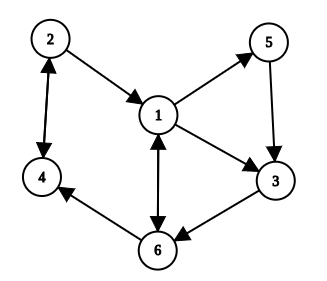
\includegraphics[scale=0.8]{images/directed_graph_example.png}
	\caption{Παράδειγμα κατευθυνόμενου γράφου \\ κατασκευάστηκε με: https://csacademy.com/app/graph\_editor/}
\end{matlab} 

Ο ορισμός για το μη κατευθυνόμενο γράφημα περιλαμβάνει ένα σύνολο \(V\) και ένα σύνολο πολυσυνόλων δύο στοιχείων \(E\). Το \(V\) αποτελεί και σε αυτήν την περιπτωση το σύνολο των κορυφών και το \(E\) το σύνολο των ακμών. Μία ενδεικτική γεμετρική αναπαράσταση δίνεται στην αντίστοιχη εικόνα παρακάτω. Και σε αυτήν την περίπτωση το \(V\) είναι ένα σύνολο σημείων, ωστόσο το \(E\) είναι ένα σύνολο γραμμών που δεν υποδικνύουν καμμία κατεύθυνση. \\

\begin{matlab}
	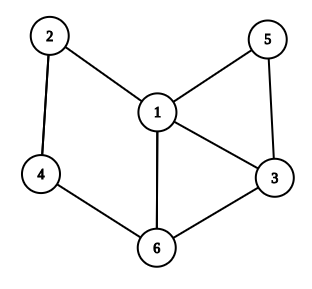
\includegraphics[scale=0.8]{images/undirected_graph_example.png}
	\caption{Παράδειγμα μη κατευθυνόμενου γράφου \\ κατασκευάστηκε με: https://csacademy.com/app/graph\_editor/}
\end{matlab}   

\subsection{Μονοπάτια}

Σε κάθε κατευθυνόμενο γράφημα οι ακμές περιέχουν μία αρχική κορυφή και μία τερματική κορυφή. Για παράδειγμα η ακμή (1,3) της εικόνας 3.1 περιέχει δύο κορυφές. Η κορυφή 1 καλείται αρχική κορυφή και η κορυφή 3 καλείται τερματική κορυφή. \\

Στα κατευθυνόμενα γραφήματα, μία ακολουθία ακμών \((e_1, e_2,...,e_k)\) όπου η τερματική κορυφή μίας ακμής \(e_j\) ταυτίζεται με την αρχική κορυφή της \(e_{(j+1)}\) καλείται μονοπάτι. \\

Αν ένα μονοπάτι δεν περιέχει την ίδια ακμή δύο φορές ονομάζεται απλό μονοπάτι. \\

Στοιχειώδες μονοποάτι καλείται το μονοπάτι εκείνο όπου δεν περιέχει την ίδια κορυφή παραπάνω από μία φορά. \\

Κύκλωμα καλείται το μονοπάτι \((e_1, e_2,...,e_k)\), όπου η τερματική κορυφή της \(e_k\) ακμής συμπίπτει με την αρχική κορυφή της \(e_1\) ακμής. \\

\subsection{Χαμιλτόνειοι κύκλοι και μονοπατια}

O Ιρλανδός φυσικός και μαθηματικός William Rowan Hamilton (4 Αυγούστου 1805 – 2 Σεπτεμβρίου 1865) μελέτησε εκτός των άλλων και τα γραφήματα. Συγκεκριμένα, δημιούργησε το μαθηματικό παιχνίδι "ο γύρος του κόσμου", του οποίου σκοπός ήταν η εύρεση ενός μονοπατιού από ακμές δωδεκαέδρου. Το μονοπάτι έπρεπε να περνά από κάθε κορυφή του δωδεκαέδρου ακριβώς μία φορά. Πιο συγκεκριμένα, ο ένας παίκτης κάρφωνε από μία βελόνα σε 5 διαδοχικές κορυφές και έπειτα ο άλλος παίκτης έπρεπε να συμπληρώσει το κύκλωμα έτσι ώστε να περιλαμβάνει όλες τις κορυφές. Μάλιστα, σε επιστολή προς τον φίλο του John T. Graves (17 Οκτωβρίου 1856) ο Hamilton τον πληροφορεί σχετικά με ένα παιχνίδι που βασίζεται στον εικοσιανό λογισμό (αλγεβρική δομή για τον υπολογισμών συμμετριών του εικοσαέδρου από τον ίδιο τον Hamilton) και την αναγνωρισιμότητα που έχει λάβει από μερικούς νεαρούς. Το παιχνίδι αυτό στάθηκε η αφορμή για την ανάπτυξη της θεωρίας γύρω από τα γραφήματα και προς τιμήν του Hamilton και του εν λόγω παιχνιδιού που επινόησε οι Χαμιλτονειανοί κύκλοι έλαβαν το όνομά του. \\

\begin{matlab}
	\includegraphics[scale=0.2]{images/Hamilton.png}
	\caption{William Rowan Hamilton \\ πηγή: https://en.wikipedia.org/wiki/William\_Rowan\_Hamilton}
\end{matlab}  

Η εύρεση ενός μονοπατιού ή ενός κυκλώματος που περνά από κάθε κορυφή ενός δεδομένου γραφήματος μόνο μία φορά φαντάζει αρχικά απλή υπόθεση, ωστόσο οι μέχρις στιγμής επιστημονικές προσεγγίσεις αποδεκνύουν το αντίθετο. 

Μονοπάτι (ή κύκλωμα) Hamilton είναι ένα μονοπάτι (ή ένα κύκλωμα) που περνά από όλες τις κορυφές ενός γραφήματος ακριβώς μία φορά. \\

Ένα γράφημα που περιέχει κύκλο Hamilton καλείται χαμιλτόνειο, ενώ αν δεν περιέχει καλείται μη χαμιλτόνειο. \\

Δυστυχώς, μέχρι και τώρα δε γνωρίζουμε κάποια ικανή και αναγκάια συνθήκη για την ύπαρξη μονοπατιών και κυκλωμάτων Hamilton. Δοθέντος ενός γραφήματος G, η απόδειξη ύπαρξης ή μη ενός μονοπατιού ή κυκλώματος Hamilton είναι η κατασκευή του. \\ 

\section{Delaunay Τριγωνοποίηση}

Στη υπολογιστική γεωμετρία, η τριγωνοποίηση πολυγώνων είναι ένα βασικό ζήτημα μελέτης. Με το όρο τριγωνοποίηση εννοούμε την διαμέριση της περιοχής που ορίζεται από το πολύγωνο σε τρίγωνα των οποίων η ένωση παράγει την περιοχή του αρχικού πολυγώνου. \\

Ουσιαστικά, η τριγωνοποίηση ενός συνόλου σημείων στο επίπεδο είναι ένα σύνολο τριγώνων. Η ένωση των τριγώνων αυτών ισούται με το κυρτό περίβλημα των σημείων και η τομή δύο τριγώνων μπορεί να είναι είτε κενή, είτε να είναι ίση με την κοινή κορυφή των δύο τριγώνων ή με την κοινή τους ακμή.

\begin{matlab}
	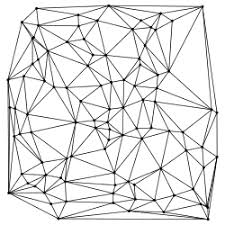
\includegraphics[scale=0.9]{images/delaunay_trianglulation.jpeg}
	\caption{Τριγωνοποίηση Delaunay \\ πηγή: https://en.wikipedia.org/wiki/Delaunay\_triangulation}
\end{matlab}

Στην παρούσα υποενότητα θα αναφερθούμε στη Delaunay τριγωνοποίηση, καθώς θα μας φανεί χρήσιμη στη μελέτη του προβλήματος του περιοδεύοντος πωλητή, με τρόπο που περιγράφεται σε επόμενη ενότητα. Επισημαίνουμε τη βασική θεωρία γύρω από την εν λόγω τριγωνοποίηση και μερικούς θεμελιώδεις αλγορίθμους που την παράγουν. \\

\subsection{Ιστορία}

Η delaunay τριγωνοποίηση ήταν μία επινόηση του Ρώσου μαθηματικού Boris Nikolaevich Delone. Ο Delone γεννήθηκε στις 15 Μαρτίου του 1890 και πέθανε έπειτα από 90 χρόνια, στις 17 Ιουλίου του 1980. Ο Boris Delone ασχολήθηκε με την άλγεβρα και τη γεωμετρία και μία από τις σημαντικότερες ανακαλύψεις του ήταν η τριγωνοποίηση Delaunay το 1934. \\

Η τριγωνοποίηση έλαβε το όνομα Delaunay, προς τιμήν του δημιουργού της, ο οποίος καλούσε τον εαυτό του "Boris Nikolaeviq Delone". Καθώς την εποχή εκείνη οι δύο επικρατέστερες γλώσσες στους επιστημονικούς κόλπους ήταν τα γαλλικά και τα γερμανικά, επικράτησε η γαλλική εκδοχή του ονόματός του και έτσι η τριγωνοποίηση έλαβε τελικά το όνομα Delaunay. \\

\begin{matlab}
	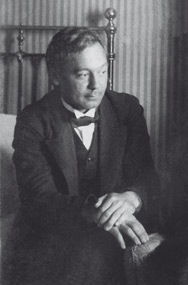
\includegraphics[scale=0.9]{images/Delone.jpg}
	\caption{Boris Nikolaevich Delone \\ πηγή: https://en.wikipedia.org/wiki/File:Delone\_cropped\_1924.jpg}
\end{matlab} 

\subsection{Βασική θεωρία}

Στόχος της τριγωνοποίησης Delaunay είναι με βάση ένα σύνολο σημείων στο επίπεδο να παράξει μία τριγωνοποίηση αυτών, η οποία να ικανοποιεί ορισμένες συνθήκες. \\

Για να μελετήσουμε την τριγωνοποίηση Delaunay πρέπει εξ αρχής να κάνουμε την παραδοχή ότι τα σημεία που πρόκειται να τριγωνοποιηθούν βρίσκονται σε γενική θέση. Γενική θέση στην παρούσα ενότητα εννοούμε ότι τέσσερα σημεία δε βρίσκονται πάνω στον ίδιο κύκλο.   \\

Αρχικά, εισάγουμε την απαραίτητη έννοια του "διανύσματος γωνιών" (vector angle). Έστω ότι \(P := \left\{ p_1, p_2,...,p_n \right\}\) είνα ένα σύνολο \(n\) σημείων στο επίπεδο. Επίσης, έστω ότι \(Τ\) είναι μια τριγωνοποίησή τους. Αν \(m\) είναι το σύνολο των τριγώνων που έχουν παραχθεί στη συγκεκριμένη τριγωνοποίηση, τότε με προφανή τρόπο εξάγεται το συμπέρασμα ότι το σύνολο των γωνιών που περιέχει η τριγωνοποίηση είναι \(3m\). Τοποθετούμε τις γωνίες της τριγωνοποίησης σε ένα διάνυσμα σε αύξουσα σειρά. Το διάνυσμα αυτό καλείται vector-angle και ορίζεται ως εξής

\begin{align}
	A(T) := (a_1, a_2, ..., a_{3m})
\end{align}   

όπου

\begin{align}
	a_i \leq a_j \text{, } \forall i<j
\end{align}

Αν \(Τ'\) είναι μια διαφορετική τριγωνοποίηση από την \(Τ\) για το ίδιο σύνολο σημείων \(P\) και το αντίστοιχο διάνυσμα γωνιών είναι το \(A(T') = (a_{1}', a_{2}', ..., a_{3m}')\), θα λέμε ότι το διάνυσμα γωνιών της \(Τ\) τριγωνοποίησης είναι μεγαλύτερο από το διάνυσμα γωνιών της \(Τ'\) τριγωνοποίησης και θα γράφουμε \(Α(Τ) > Α(Τ')\) αν υπάρχει \(i\), όπου \(1 \leq i \leq 3m\) τέτοιο ώστε 

\begin{align*}
	a_j = a_{j}' \text{, } \forall j < i \text{ και } a_i > a_{i}'
\end{align*}

Θα δούμε στη συνέχεια ότι στόχος μας εδώ είναι να καταφέρουμε να εντοπίσουμε το μεγαλύτερο διάνυσμα γωνιών. \\

Θα λέμε ότι μία τριγωνοποίηση είναι "angle-optimal" και θα γράφουμε \(Α(Τ) \geq A(T')\) αν \(Α(Τ) > Α(Τ')\) για όλες τις δυνατές τριγωνοποιήσεις \(T'\). \\

Στο σημείο αυτό πρέπει να αναφέρουμε ότι το πλήθος των τριγώνων που προκύπτουν από μία τριγωνοποίηση δεν είναι τυχαίο. Μπορεί να καθοριστεί με ακρίβεια, πράγμα που ήδη έχει διατυπωθεί σε αντίστοιχο θεώρημα. \\

\begin{mytheorem}{Πλήθος ακμών και τριγώνων τριγωνοποίησης σημείων στο επίπεδο}{Α}
	Έστω \(P\) ένα σύνολο \(n\) σημείων στο επίπεδο. Έστω ότι τα σημεία δεν είναι όλα μεταξύ τους συνευθειακά και έστω με \(k\) να συμβολίζονται ότα τα σημεία που βρίσκονται στο όριο του convex hull του \(P\). Οποιαδήποτε τριγωνοποίηση των σημείων του \(P\) παράγει \(2n - 2 - k \) τρίγωνα και \(3n - 3 - k\) ακμές.
\end{mytheorem}

Απόδειξη: \\
Έστω ότι τα \(P\) σημεία τριγωνοποιούνται και παράγονται \(m\) το πλήθος τρίγωνα. Συνεπώς, το επίπεδο έχει διαχωριστεί με \(m + 1\) υποπεριοχές. \\
Κάθε τρίγωνο έχει 3 ακμές και το convex hull έχει \(k\) ακμές. \\
Κάθε ακμή ανήκει σε δύο υποπεριοχές του επιπέδου. \\
Συνεπώς, ο συνολικός αριθμός ακμών είναι  \(\frac{3m + k}{2}\). \\
Από τον τύπο του Euler, όπου \(n_f = m + 1\) και \(n_e = \frac{3m + k}{2}\), προκύπτει ότι 

\begin{align*}
	n - n_e + n_f= 2 & \Leftrightarrow \\
	n - \frac{3m + k}{2} + (m+1) = 2 & \Leftrightarrow \\	
	2n - (3m + k) + 2(m+1) = 4 & \Leftrightarrow \\
	2n - 3m - k + 2m + 2 = 4 & \Leftrightarrow \\
	2n - m - k = 2 & \Leftrightarrow \\
	m = 2n - k - 2
\end{align*}

και αφού \(m = 2n - 2 - k\), το \(n_e\) υπολογίζεται να είναι

\begin{align*}
	n_e = \frac{3m + k}{2} & \Leftrightarrow \\
	n_e = \frac{3(2n - k - 2) + k}{2} & \Leftrightarrow \\
	n_e = \frac{6n - 3k - 6 + k}{2} & \Leftrightarrow \\
	n_e = \frac{6n - 6 - 2k}{2} & \Leftrightarrow \\
	n_e = 3n - 3 - k
\end{align*}

\(\square \)

Όπως ήδη αναφέραμε στόχος είναι να βρεθεί η τριγωνοποίηση που δίνει το "μεγαλύτερο" διάνυσμα γωνιών. Για να καταφέρουμε να φτάσουμε στο σημείο να παράξουμε μία τέτοια τριγωνοποίηση για ένα δεδομένο σύνολο σημείων πρέπει να αναφέρουμε μερικές ακόμα θεμελιώδεις έννοιες. Εισάγουμε την έννοια της "παράνομης ακμής" (illegal edge). \\

Έστω μία τριγωνοποίηση των \(P\) σημείων και έστω μία ακμή της τριγωνοποίησης που βρίσκεται εντός ενός κυρτού τετράπλευρου και είναι κοινή ακμή για δύο διαφορετικά τρίγωνα της τριγωνοποίησης. Η ακμή αυτή μπορέι να γίνει flip. Στην περίπτωση αυτή το μόνο που αλλάζει είναι το \(A(T)\). \\

\begin{mydefinition}{Παράνομη ακμή}{α}
	Έστω \(T\) μία τριγωνοποίηση των σημείων \(P\).  Καλούμε μία ακμή "παράνομη" εαν μπορούμε να αυξήσουμε τη μικρότερη γωνία του διανύσματος γωνιών κάνοντάς την flip.
\end{mydefinition}

Αν \(T\) μία τριγωνοποίηση που περιέχει μία παράνομη ακμή και \(T'\) η τριγωνοποίηση που έχει γίνει flip η παράνομη ακμή, τότε ισχύει ότι η \(T'\) είναι angle-optimal:

\begin{align*}
	A(T') \geq A(T)
\end{align*}

\begin{mydefinition}{}{}
	Μία τριγωνοποίηση \(T\) καλείται νόμιμη εαν δεν περιέχει καμία παράνομη ακμή.
\end{mydefinition}

Συνεπώς, κάθε angle-optimal τριγωνοποίηση είναι νόμιμη. \\

Με βάση αυτήν την τεχνική μπορούμε να οδηγηθούμε σε μία τριγωνοποίηση Delaunay. \\

\begin{mydefinition}{Τριγωνοποίηση Delaunay}{}
	Για ένα σύνολο σημείων \(P\) στο επίπεδο, η τριγωνοποίηση Delaunay είναι η τριγωνοποίηση εκείνη που δεν περιέχει καμία παράνομη ακμή. Συμβολίζουμε την τριγωνοποίηση Delaunay των σημείων με \(Del(P)\).
\end{mydefinition}

Μία εναλλακτική προσέγγιση των flips και των ελέγχων των διανυσμάτων γωνιών για την παραγωγή Delaunay τριγωνοποίησης είναι η προσέγγιση με τη βασικό εργαλείο τον κύκλο. Στο σημείο αυτό, επισημαίνουμε κάποιες βασικές ιδιότητες που αφορούν τον κύκλο και πηγάζουν από το θεώρημα του Θαλή. \\

\begin{matlab}
	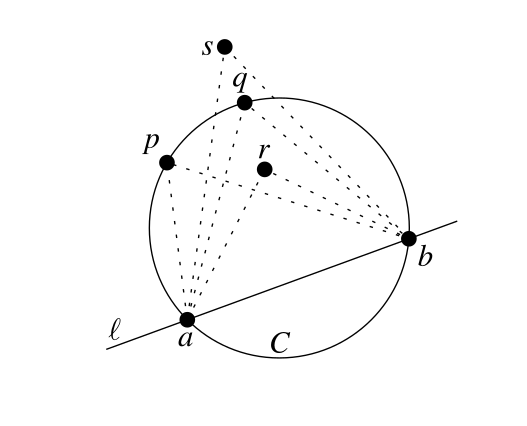
\includegraphics[scale=0.4]{images/circle.png}
	\caption{Κύκλος C με τόξο ab \\ πηγή: "Computational Geometry, Algorithms and Applications,Third Edition", σελ. 194}
\end{matlab}

\begin{mytheorem}{Γωνίες που βαίνουν σε χορδή}{χορδη1}
	Έστω \(C\) να είναι ένας κύκλος και \(l\) μία ευθεία που τέμνει τον κύκλο στα σημεία \(a\) και \(b\). Έστω \(p\) και \(q\) σημεία πάνω στην περίμετρο του κύκλου. Τότε η γωνία που βαίνει στο τόξο \(ab\) με κορυφή το σημείο \(p\) είναι ίση με την γωνία που βαίνει στο ίδιο τόξο και έχει κορυφή το σημείο \(q\). 
\end{mytheorem}

\begin{mytheorem}{Γωνίες που βαίνουν σε χορδή}{χορδη2}
	Έστω \(C\) να είναι ένας κύκλος και \(l\) μία ευθεία που τέμνει τον κύκλο στα σημεία \(a\) και \(b\). Έστω \(r\) ένα σημείο εντός του κύκλου και \(s\) ένα σημείο εκτός. Τότε η γωνία που βαίνει στο τόξο \(ab\) με κορυφή το σημείο \(r\) είναι μεγαλύτερη από την γωνία που βαίνει στο ίδιο τόξο και έχει κορυφή το σημείο \(s\). 
\end{mytheorem}

Συνοψίζοντας 

\begin{align}
	\angle arb > \angle apb = \angle aqb > \angle asb
\end{align}

Από όλα τα παραπάνω προκύπτει ότι \\

\begin{mylemma}{}{}
	Έστω \(C\) ένας κύκλος και \(p_i, p_j, p_k\) σημεία πάνω στον κύκλο και \(p_l\) σημείο εντός του κύκλου. Αν τα \(p_i, p_j, p_k, p_l\) σχηματίζουν ένα κυρτό πολύγωνο, τότε αυτό μπορεί να τριγωνοποιηθεί και να παραχθούν τα τρίγωνα \(p_i p_j p_k\) και \(p_i p_j p_l\) με κοινή ακμή την \(p_i p_j\). Η ακμή \(p_i p_j\) είναι παράνομη.
\end{mylemma} 

\begin{mylemma}{}{}
	Έστω \(C\) ένας κύκλος και \(p_i, p_j, p_k\) σημεία πάνω στον κύκλο και \(p_l\) σημείο εκτός του κύκλου. Αν τα \(p_i, p_j, p_k, p_l\) σχηματίζουν ένα κυρτό πολύγωνο, τότε αυτό μπορεί να τριγωνοποιηθεί και να παραχθούν τα τρίγωνα \(p_i p_j p_k\) και \(p_i p_j p_l\) με κοινή ακμή την \(p_i p_j\). Η ακμή \(p_i p_j\) είναι νόμιμη.
\end{mylemma} 

Φυσικά, να υπενθυμίσουμε ότι τα σημεία βρίσκονται σε γενική θέση, συνεπώς δεν παίρνουμε την περίπτωση τα \(p_i, p_j, p_k, p_l\) να είναι και τα 4 πάνω στον ίδιο κύκλο. \\

Στο παραακάτω θεώρημα συνοψίζεται η προσέγγιση της τριγωνοποίησης με εργαλείο τον κύκλο. \\

\begin{mytheorem}{Η ιδιότητα των κενών κυκλων}{}
	Έστω \(P\) ένα σύνολο σημείων στο επίπεδο που βρίσκονται σε γενική θέση. Μία τριγωνοποίηση \(T\) είναι τριγωνοποίηση Delaunay αν και μόνο αν ο κυκλος που σχηματίζεται από κάθε τριάδα σημείων που αποτελούν τρίγωνο της τριγωνοποίησης δεν περιέχει κανένα άλλο σημείο του \(P\) στο εσωτερικό του.
\end{mytheorem} 

Απόδειξη: \\
\(\Rightarrow \) \\
Αν κανένα σημείο του συνόλου σημείων \(P\) δεν βρίσκεται εσωτερικά του εκάστοτε κύκλου που σχηματίζεται από τις τρεις κορυφές ενός τριγώνου της τριγωνοποίησης, τότε όλες οι ακμές είναι νόμιμες. Συνεπώς, η τριγωνοποίηση είναι νόμιμη. \\
\(\Leftarrow \) "Αν μια τριγωνοποίηση είναι Delaunay, τότε κανένα σημείο του \(P\) δεν βρίσκεται εντός του εκάστοτε κύκλου τριών κορυφών τριγώνου της τιγωνοποίησης" \\
Θα αποδείξουμε αυτήν την κατεύθυνση με απαγωγή σε άτοπο. \\
Έστω ότι η τριγωνοποίηση \(T\) είναι τριγωνοποίηση Delaunay και έστω ότι υπάρχει κύκλος που περιέχει σημεία του \(P\) εκτός των \(A, B, C\) που τον ορίζουν και είναι οι κορυφές ενός τριγώνου της τριγωνοποίησης. \\
Έστω ότι από όλα αυτά τα σημεία επιλέγεται εκείνο που απέχει την μικότερη απόσταση απο την ακμή του τριγώνου, έστω \(D\). \\
Επειδή η τριγωνοποίηση είναι Delaunay, το τρίγωνο \(BCD\) δε μπορεί να ανήκει στην τριγωνοποίηση. \\
Έστω \(Ε\) ένα σημείο εκτός του κύκλου και \(BCE\) τρίγωνο. Το \(D\) βρίσκεται εντός του κύκλου που ορίζεται από τα σημεία \(B, C, E\) και εκτός του τριγώνου \(BCE\). 
......................................

\begin{matlab}
	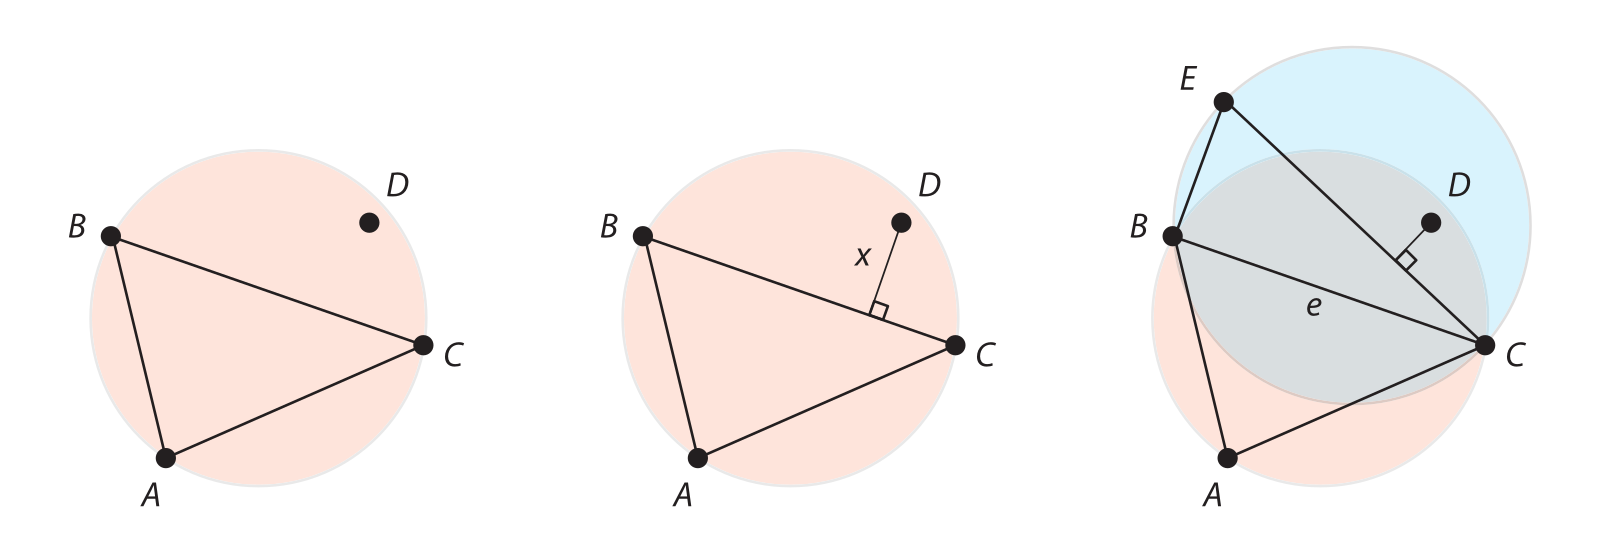
\includegraphics[scale=0.3]{images/emptycircle.png}
	\caption{Απόδειξη του θεωρήματος 3.2.4 \\ πηγή: "Discrete and Computational Geometry", σελ.: 86}
\end{matlab} 

Συνοψίζουμε τα κριτήρια για την Delaunay τριγωνοποίηση σε ένα θεώρημα. \\

\begin{mytheorem}{Delaunay Τριγωνοποίηση}{}
	Σε μία τριγωνοποίηση Delaunay \(T\) των σημείων \(P\): \\
	1. Τρία σημεία κατασκευάζουν τρίγωνο αν και μόνο αν ο περιγεγραμμένος ανοιχτός κύκλος του δεν περιέχει κανένα άλλο σημείο του \(P\). \\
	2. Δύο σημεία κατασκευάζουν ακμή αν και μόνο αν υπάρχει κύκλος με τα σημεία αυτά στην περιφέρειά του που δεν περιέχει κανένα άλλο σημείο του \(P\) 	
\end{mytheorem}

Για δεδομένη τριγωνοποίηση, θα αποφασίζουμε αν αυτή είναι Delaunay ανν ο περιγεγραμμένος κύκλος κάθε τριγώνου δεν περιέχει κανένα άλλο σημείο. \\

\subsection{Κατασκευή Delaunay Τριγωνοποίησης}

Αφού είδαμε τη θεωρητική βάση της τριγωνοποίησης Delaunay, μπορούμε πλέον να αναφερθούμε σε τεχνικές και αλγόριθμους που κατασκευάζουν μία τριγωνοποίηση Delaunay. \\

\subsubsection{Αυξητκός αλγόριθμος}

Ο αλγόριθμος αυτός δε γνωρίζει εκ των προτέρων όλα τα σημεία που πρόκειται να τριγωνοποιηθούν. Για τη ακρίβεια, λαμβάνει ένα σύνολο σημείων, σε κάθε βήμα του εξετάζει ενα απο τα σημεία αυτά και παράγει την τρέχουσα Delaunay τριγωνοποίηση σαν να μην υπάρχουν άλλα σημεία προς εξέταση, μέχρι που εξετάζει όλο το σύνολο σημείων και παράγει της τελική Delaunay τριγωνοποίηση. Η επιλογή σημείου σε κάθε βήμα γίνεται με τυχαίο τρόπο. \\

Ο αλγόριθμος έχει \(Ο(n logn)\) μέση πολυπλοκότητα, ενώ στη χείριστη περίπτωση η πολυπλοκότητά του είναι \(O(n^2)\). \\

Ο αλγόριθμος επιλέγει 3 σημεία στο επίπεδο των οποίων το αντίστοιχο τρίγωνο περιλαμβάνει όλα τα σημεία προς τριγωνοποίηση. Η επιλογή των τριών αυτών σημείων δεν είναι τυχαία και πρέπει να πληρεί ορισμένα κριτήρια. Θα αναφερθούμε σε αυτά στη συνέχεια, αφού πρώτα παρουσιάσουμε τον πυρήνα του αλγορίθμου. \\

Ο αλγόριθμος αυξητικά παράξει σε κάθε του βήμα την τριγωνοποίηση. Για κάθε σημείο που ελέγχει εντόπίζει αν βρίσκεται εντός τριγώνου της ήδη κατασκευασμένης τριγωνοποίησης ή πάνω σε κάποια ακμής της τριγωνοποίησης. Στην περίπτωση που βρίσκεται μέσα σε τρίγωνο κατασκευάζονται τρείς νέες ακμές, οι οποίες εκτείνονται από το υπό εξέταση σημείο προς την κάθε κορυφή του τριγώνου που το περιέχει. Στην περίπτωση που το σημείο βρίσκεται πάνω σε ακμή της τριγωνοποίησης είναι εύκολο κανείς να συνειδητοποιήσει ότι η ακμή αυτή είναι κοινή ακμή για δύο τριγωνα. Συνεπώς, δημιουργούνται δύο νέες ακμές από το σημείο που εξετάζεται προς τη μία κορυφη του ενός και του άλλου τριγώνου που δεν ανήκουν στο ευθύγραμμο τμήμα. Για την καλύτερη κατανόηση των δύο περιπτώσεων παρέχεται η αντίστοιχη εικόνα. Αφού δημιουργηθούν οι νέες ακμές με κατάλληλο τρόπο μένει να ελέγξουμε ότι η τριγωνοποίηση που έχει παραχθεί είναι Delaunay. Η προσθήκη μιας νέας ακμής μπορεί να κάνει παράνομες τις ήδη υπάρχουσες ακμές της τριγωνοποίησης. Αυτο αντιμετωπίζεται με κατάλληλα flips κάθε φορά. Ο αλγόριθμος παρουσιάζεται συνοπτικά παρακάτω. \\

Ο αλγόριθμος σαφώς τερματίζει, καθώς το πλήθος των ακμών της τριγωνοποίησης είναι πεπερασμένο. Επίσης, ο αλγόριθμος είναι ορθός διότι εξετάζει κάθε ακμή ως προς την "νομιμότητά" της στο βήμα όπου καλεί τον αλγόριθμο "Νομιμοποίηση ακμής". Συνεπώς, ποτέ δε θα προκύψει παράνομη ακμή χωρίς να ελεγχθεί και να μετατραπεί σε νόμιμη. όπως ήδη έχουμε αναφέρει, μια τριγωνοποίηση είναι Delaunay αν είναι νόμιμη. \\

\begin{algorithm}[H]
	\SetAlgoLined
	\KwIn{n σημεία του επιπέδου}
	\KwResult{Τριγωνοποίηση Delaunay για n σημεία του επιπέδου}
	
	Δημιούργησε κατάλληλα σημεία \(p_{-1}, p_{-2}, p_{-3}\) στο επίπεδο έτσι ώστε το τρίγωνο που σχηματίζουν να περέχει τα n σημεία εισόδου. \;
	\For{ένα σημείο του επιπέδου που δεν έχει ενταχθέι στην τριγωνοποίηση}
	{Βρες σε ποιο τρίγωνο ή ακμή ανήκει \;
	\If{σημείο ανήκει σε τρίγωνο}
		{Πρόσθεσε 3 νέες ακμές προς τις κορυφές του τριγώνου \;
		Κάλεσε τον αλγόριθμο 2 για τις 3 πλευρές του τριγώνου \;}
	\Else
		{Πρόσθεσε 2 νέες ακμές προς τις κορυφές των τριγώνων που έχουν κοινή πλευρά την πλευρά που ανήκει το υπο εξέταση σημείο \;
		Κάλεσε τον αλγόριθμο 2 για τις 4 πλευρές των 2 τριγώνων \;}
	}	
	
	\caption{Αυξητικός αλγόριθμος τριγωνοποίησης Delaunay}
\end{algorithm}

\begin{algorithm}[H]
	\SetAlgoLined
	\KwIn{Τριγωνοποίηση σημείων, ακμή της τριγωνοποίησης \(p_i p_j\), σημείο \(p_r\)}
	\KwResult{Τριγωνοποίηση που είναι νόμιμη}
	
	Βρές τρίγωνο \((p_i, p_j, p_l)\) \;
	\If{\(p_i p_j\) παράνομη}
	{Διαγραφή \(p_i p_j\) \;
	Δημιουργία \(p_r p_l\) \;
	\(p_i p_l\) = νόμιμη ως προς την \(p_r\) \;
	\(p_j p_l\) = νόμιμη ως προς την \(p_r\) \;}
	
	\caption{Νομιμοποίηση ακμής}
\end{algorithm}

\begin{matlab}
	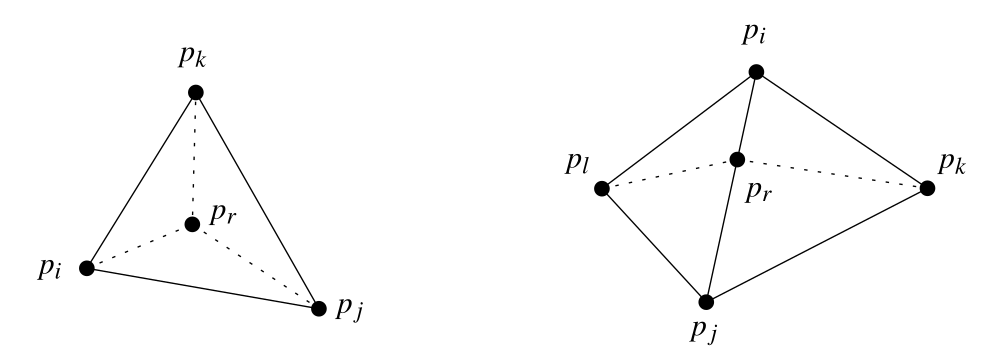
\includegraphics[scale=0.3]{images/incremental.png}
	\caption{Οι δύο περιπτώσεις που εξετάζει ο αυξητικός αλγόριθμος κατά την εισαγωγή ενός νέου σημείου \(p_r\). Αριστερά φαίνεται η πρώτη περίπτωση, όπου το νεό σημείο εντοπίζεται εντός τριγώνου της τριγωνοποίησης, ενώ δεξία φαίνεται η δεύτερη περίπτωση όπου το νέο σημείο βρίσκεται πάνω σε ακμή της τριγωνοποίησης \\ πηγή: "Computational Geometry, Algorithms and Applications, Third Edition", σελ.: 200}
\end{matlab} 

Στο σημείο αυτό μπορούμε να εξηγήσουμε τον τρόπο που επιλέγουμε τα τρία αρχικά σημεία που δημιουργούν τρίγωνο που περιβάλει όλα τα προς τριγωνοποίηση σημεία. Ουσιαστικά, τα σημεία αυτά πρέπει να λάβουν θέσεις στο επίπεδο, που να μην επηρεάζουν την έκβαση της τριγωνοποίσης μετέπειτα. Αυτό επιτυγχάνεται μόνο αν τοποθετηθούν αρκετά μακρυά από τα σημεία που πρόκειται να τριγωνοποιηθούν. Για να συμβεί αυτό πρέπει καθένα από τα σημεία \(p_{-1}, p_{-2}, p_{-3}\) να μην βρίσκονται εντός των κύκλων που σχηματίζονται από όλες τις δυνατές τριάδες σημειων. Μόνο τότε μπορούμε να είμαστε βέβαιοι ότι δεν έχουν επηρεάσει την τριγωνοποίηση Delaunay. \\

Τέλος, πρέπει να αποσαφηνίσουμε τον τρόπο με τον οποίον ο αλγόριθμος αντιλαμβάνεται πότε ένα σημείο είναι εντός τριγώνου ή πάνω σε κάποια ακμή. Αυτό επιτυγχάνεται με τη δημιουργία ενός κατάλληλου κατευθυνόμενου ακυκλικού γράφου. Ο γράφος αυτός κωδικοποιεί όλα τα τρίγωνα που δημιουγήθηκαν κατά την εκτέλεση του αλγορίθμου και την χρονική τους ιεραρχία. Οι κόμβοι είναι τρίγωνα και οι ακμές δηλώνουν τις σχέσεις μεταξύ δύο τριγώνων. Αν δύο κόμβοι συνδέονται με ακμή, δηλαδη με σχέση "πατέρα - παιδιού", τότε τα αντίστοιχα τρίγωνα έχουν μη κενή τομή. Είναι προφανές πως η ρίζα του γράφου είναι το τρίγωνο \(p_{-1} p_{-2} p_{-3}\). Έχουμε ήδη αναφέρει ότι η προσθήκη ενός νέου σημείου μπορεί να δημιουργήσει τρία ή τέσσερα τρίγωνα στην τριγωνοποίηση. Σε όρους γράφου, αυτό σημαίνει τρία ή τέσσερα νέα φύλλα. Το flip μιας ακμής δημιουργεί μόνο δύο φύλλα. \\

Για τον εντοπισμό ενός σημείου, διατρέχεται ο γράφος ξεκινόντας από τη ρίζα. Ελέγχονται τα τρία παιδία της ρίζας και εντοπίζουμε σε ποιο από αυτά τα τρία τρίγωνα (που περιέχονται στους κόμβους) ανήκει το προς εξέταση σημείο. Μεταβαίνουμε στο κατάλληλο παιδί και συνεχίζουμε την ίδια ακριβώς διαδικασία μέχρι να φτάσουμε σε φύλλο του γράφου στο οποίο και εντοπίζεται το σημείο που εξετάζουμε. \\ 

\chapter{Γραφοθεωρητική Προσέγγιση του Προβλήματος του πλανόδιου πωλητή}
 
Η προσέγγιση του TSP με βάση τη θεωρία γραφημάτων συνδέεται στενά με τα τους Χαμιλτόνειους κύκλους. Επί της ουσίας το πρόβλημα του περιοδεύονοτς πωλητή είναι μία επέκταση του προβλήματος εύρεσης κυκλώματος Hamilton. \\ 

Όπως ήδη έχουμε αναφέρει στην εισαγωγή, στόχος του προβλήματος είναι ο πωλητής να επισκεφτεί ένα σύνολο πόλεων, ακριβώς μία φορά την κάθε μία, ελαχιστοποιόντας τις αποστάσεις που πρέπει να διανύσει. Αν αναπαραστήσουμε το σύνολο των πόλεων προς επίσκεψη με ένα σύνολο κορυφών \(V\) και το σύνολο όλων των πιθανών διαδρομών με ενα σύνολο \(E\), τότε μπορούμε να μεταφέρουμε την εικόνα του χάρτη που μελετά ο πωλητής σε γραφική αναπαράσταση. Ο πωλητής εκκινεί και τερματίζει το ταξίδι του στην ίδια πόλη και επισκέπτεται όλες τις υπόλοιπες ακριβώς μία φορά, διανύοντας το έλαχιστον συνολικό μήκος. \\

Θεωρούμε το παραπάνω γράφημα του χαρτη των πόλεων και των αντίστοιχων διαδρομών να είναι το \(G = (V,E,w(i,j))\), όπου το \(V\) περιλμβάνει τις \(n\) πόλεις  (κορυφές), το \(E\) τις διαδρομές μεταξύ δύο πόλεων (ακμές) και το \(w\) να είναι μία συνάρτηση 

\begin{align}
	w:E \rightarrow \R^{+}
\end{align} 
 
τέτοια ώστε να ισχύει 

\begin{align}
	w(i,k) \leq w(i,j) + w(j,k)
\end{align} 

Ουσιαστικά το \(w(i,j)\) είναι το μήκος της διαδρομής από την πόλη \(i\) στην πόλη \(j\) ή με όρους γραφημάτων το βάρος της ακμής \((i,j)\). Στην περίπτωση κυκλώματος, το μήκος του ορίζεται να είναι το άθροισμα των μηκών των αντίστοιχν ακμών. \\

Το TSP αναζητά ένα κύκλωμα Hamilton με ελάχιστο μήκος. Δυστυχώς, μέχρι και σήμερα δε γνωρίζουμε κανέναν αλγόριθμο που να επιλύει το πρόβλημα του περιοδεύοντος πωλητή για μερικές εκατοντάδες πόλεων σε εύλογα χρονικά πλαίσια. \\

\section{Η μέθοδος του πλησιέστερου γείτονα}

Μία πολύ απλή μέθοδος για την εύρεση Χαμιλτονειανού κύκλου σε ένα γράφημα \(G = (V,E,w(i,j))\) είναι η μέθοδος του πλησιέστερου γείτονα. 

\begin{algorithm}[H]
	\SetAlgoLined
	\KwResult{Κύκλωμα Hamilton για το πρόβλημα του περιοδέυοντος πωλητή}
	
	Επέλεξε αυθαίρετα μία κορυφή v \;
	Ανέθεσε την v στην x \;
	\For{x} 
	{Επέλεξε μία κορυφή v που δεν βρίσκεται στο μονοπάτι και απέχει τη μικρότερη απόσταση από την τρέχουσα x \;
	Πρόσθεσε την ακμή (x,v) στο μονοπάτι \;
	Ανανέωσε την x με την v \;}
	Σχημάτισε κύκλωμα συνδέοντας την αρχική κορυφή με την τελική κορυφή του μονοπατιού \;
	
	\caption{Μέθοδος πλησιέστερου γείτονα}
\end{algorithm}

\chapter{Γεωμετρική Προσέγγιση του Προβλήματος του πλανόδιου πωλητή}

\chapter{Results}

\chapter{Discussion and Future work}

\chapter{Acknowledgement}

\chapter{References}
\begin{thebibliography}{depth}
	\bibitem[1]{1}
	Exact and Approximation Algorithms for Time-Window TSP, 
	Jie Gao, Su Jia, Joseph S. B. Mitchell,
	CG:YRF, Boston, MA, USA, June 14-18, 2016
	
	\bibitem[2]{2}
	An Optimal Lower Bound for the Hilbert-type, Planar Universal Traveling Salesman Problem, 
	Patrick Eades, Julián Mestre,
	CG:YRF, Brisbane, Australia, July 4-7, 2017
	
	\bibitem[3]{3}
	The Geometric Maximum Traveling Salesman Problem, 
	David S. Johnson, Arie Tamir,
	Article in Journal of the ACM · May 2002
	
	\bibitem[4]{4}
	Εισαγωγή στους αλγορίθμους, Δεύτερη έκδοση, 
	Thomas H. Cormen, Charles E. Leiserson, Ronald L. Rivest, Clifford Stein,
	Πανεπιστημιακές εκδόσεις Κρήτης, 2011,
	ISBN: 978-960-524-473-6
	
	\bibitem[5]{5}
	Τεχνητή Νοημοσύνη, Μία σύγχρονη προσέγγιση, Δεύτερη Αμερικανική έκδοση, 
	Stuart Russel, Peter Norvig,
	σελ.: 101,
	Κλειδάριθμος 2005,
	ISBN: 960-209-873-2
	
	\bibitem[6]{6}
	Στοιχεία διακριτών μαθηματικών, 
	C. L. Liu,
	σελ.: 171-172, 178-179, 190-201,
	Πανεπιστημιακές εκδόσεις Κρήτης 2014, 
	ISBN: 978-960-524-072-1	
	
	\bibitem[7]{7}
	Discrete and Computational Geometry, 
	Satyan L. Devadoss, Joseph O'Rourke,
	σελ.: 81-86,
	Princeton University Press, 2011, 
	ISBN: 978-0-691-14553-2
	
	\bibitem[8]{8}
	Computational Geometry,	Algorithms and Applications, Third Edition, 
	Mark de Berg, Otfried Cheong, Marc van Kreveld, Mark Overmars,
	σελ.: 193-204,
	Springer, 2008, 
	ISBN: 978-3-540-77973-5
	
	\bibitem[9]{9}
	Υπολογιστική Γεωμετρία: Μια σύγχρονη αλγοριθμική προσέγγιση, 
	Γιάννης Ζ. Εμίρης,
	σελ.: 199-208,
	Κλειδάριθμος, 2008, 
	ISBN: 978-960-461-141-6 
	
\end{thebibliography}
\end{document}